%%%%%%%%%%%%%%%%%%%%%%%%%%%%%%%%%%%%%%%%%%%%%%%%%%%%%%%%%%%%%%%%%%%%%%%%%%%%%%%
\chapter{Leis de Newton}
\label{Chap:ExpLeisDeNewton}
%%%%%%%%%%%%%%%%%%%%%%%%%%%%%%%%%%%%%%%%%%%%%%%%%%%%%%%%%%%%%%%%%%%%%%%%%%%%%%%

\begin{fullwidth}\it
	Realizaremos um experimento no qual dois corpos estão ligados por um fio, sendo que um deles pode se deslocar livremente no eixo vertical, enquanto o outro se desloca no eixo horizontal. Através desse aparato, poderemos calcular a aceleração através das Leis de Newton --- assumindo que podemos determinar as forças que atuam sobre o sistema, exceto pelas forças de atrito e arrasto, que devem ser desprezíveis ---. Além disso, seremos capazes de calcular a aceleração através de informações cinemáticas (distância percorrida e tempo correspondente), permitindo uma comparação entre os valores obtidos. Utilizaremos os conceitos de medidas, algarismos significativos, gráficos, regressão linear, e linearização.
\end{fullwidth}

%%%%%%%%%%%%%%%%%%%%%%%%%%%%%%%%%%%%%%%%%%%%%%%%%%%%%%%%%%%%%%%%%%%%%%%%%%%%%%%
\section{Leis de Newton}
%%%%%%%%%%%%%%%%%%%%%%%%%%%%%%%%%%%%%%%%%%%%%%%%%%%%%%%%%%%%%%%%%%%%%%%%%%%%%%%

Ao estudar o movimento dos corpos, verificamos que são necessárias três grandezas para descrever o movimento: a \emph{posição}, a \emph{velocidade} e a \emph{aceleração}. Além disso, sabemos que estas três grandezas estão relacionadas através de
\begin{align}
	\vec{v} &= \frac{d\vec{r}}{dt} \\
	\vec{a} &= \frac{d\vec{v}}{dt}.
\end{align}

Por outro lado, podemos relacionar o movimento de um corpo às forças que atuam nele através das leis de Newton, que podem ser enunciadas como:
\begin{description}
	\item[1\textordfeminine Lei] Se nenhuma força resultante atua sobre um corpo, sua velocidade não pode mudar, ou seja, o corpo não pode sofrer uma aceleração.
	\item[2\textordfeminine Lei] A força resultante que age sobre um corpo é igual ao produto da massa do corpo pela sua aceleração, isto é,
		\begin{equation}
			\vec{F}_{\textrm{res}} = m\vec{a}.
		\end{equation}
	\item[3\textordfeminine Lei] Quando dois corpos interagem, as forças que cada corpo exerce sobre o outro são sempre iguais em módulo e têm sentidos opostos.
\end{description}
%
Do ponto de vista do estudo do movimento de um corpo submetido a uma ou mais forças, as leis de Newton transferem parte do problema para a determinação de características das forças envolvidas no problema. Devido a isto, é importante conhecermos algumas características das forças mais comuns:
\begin{description}
	\item[Força Peso] A força peso a força gravitacional exercida sobre um corpo próximo à superfície da Terra, sempre em direção ao centro da Terra e com módulo dado por
	\begin{equation}
		P = mg.
	\end{equation}
	A origem de tal expressão é a lei da gravitação universal:
	\begin{equation}
		F_g = G \frac{M_T m}{r_T^2},
	\end{equation}
	onde $G = \np[N\cdot m^2/kg^2]{6,673e-11}$ é a constante da gravitação, $M_T$ é a massa da Terra e $r_T$ é o raio da Terra. Como esse último varia pouco (percentualmente), podemos reescrever a expressão acima como
	\begin{align}
		F_g &= \left[\frac{G M_T}{r_T^2}\right] m \\
			&= mg,
	\end{align}
	onde $g \approx \np[m/s^2]{9,8}$.

\item[Força Normal] A força normal ganha esse nome pois ela é sempre \emph{normal}, ou seja, \emph{perpendicular} à superfície de interação entre dois corpos quaisquer. Quando colocamos um objeto sobre uma mesa, por exemplo, ele estará sujeito à força peso --- devida a atração gravitacional exercida pela Terra sobre o objeto --- e a uma força normal exercida pela mesa sobre o objeto.
	
	Se a mesa for completamente horizontal, a força será dirigida para cima. Sobre o módulo da força, no entanto, não podemos afirmar muita coisa: sabemos que nesse tipo de situação o objeto deve permanecer parado sobre a mesa, de onde concluímos que a normal tem o mesmo módulo que o peso. Se, entretanto, o objeto for uma caixa, poderemos colocar outros objetos dentro dele e assim aumentaremos a força gravitacional exercida sobre o conjunto. Nessa situação observamos que o sistema continua em repouso, de onde concluímos que a força normal aumentou. Podemos afirmar, portanto, que a força normal pode variar em resposta a componente da força peso que é perpendicular à superfície. Por outro lado, se colocarmos uma carga exageradamente grande sobre uma mesa fraca, verificamos que a mesa quebra, portanto concluímos que a força normal deve ter um valor máximo.

	Em situações onde o objeto sobre o qual a força normal age pode ser submetido a acelerações --- dentro de um elevador, por exemplo --- temos uma situação ainda mais complexa. O valor da força normal passa também a variar dependendo do estado de aceleração do sitema elevador-objeto. Percebe-se, portanto, que a determinação exata do valor do módulo da força normal requer uma análise aprofundada da situação em questão.

\item[Tensão] A tensão tem um comportamento bastante similar ao da força normal. Se prendermos um fio ao teto de uma sala e pendurarmos um balde, verificamos que o balde permanecerá em repouso. Portanto, sabemos que a tensão equilibra a força peso. Se enchermos o balde com água, aumentamos a massa do conjunto e, consequentemente, a força peso. Ao fazer isso, no entanto, não notamos nenhum deslocamento do balde (se o fio for inextensível). Se aumentarmos muito a carga do balde, podemos fazer com que o fio atinja e ultrapasse seu valor máximo de tensão, fazendo com que ele se rompa.

	Da mesma forma que com a força normal, se tivermos uma aceleração do sistema, precisaremos leva-lá em consideração ao calcular o valor da tensão. Portanto, também precisamos de uma análise aprofundada da situação em questão.
\end{description}

%%%%%%%%%%%%%%%%%%%%%%%%%%%%%%%%%%%%%%%%%%%%
\section{Máquina de Atwood}
\label{Sec:MaquinaDeAtwood}
%%%%%%%%%%%%%%%%%%%%%%%%%%%%%%%%%%%%%%%%%%%%

Através dos conceitos expostos acima, podemos fazer uma análise do movimento horizontal de ``carrinho'' em um trilho de ar, sendo que ele é puxado através de um fio por um corpo suspenso. A Figura~\ref{FigTrilhoDeAr} mostra o aparato experimental desse experimento. Nessa configuração, o trilho de ar equivale a uma \emph{Máquina de Atwood}. Vamos analisar esse sistema de duas formas distintas, para que possamos comparar os resultados obtidos com cada uma delas.

\begin{figure}
\centering
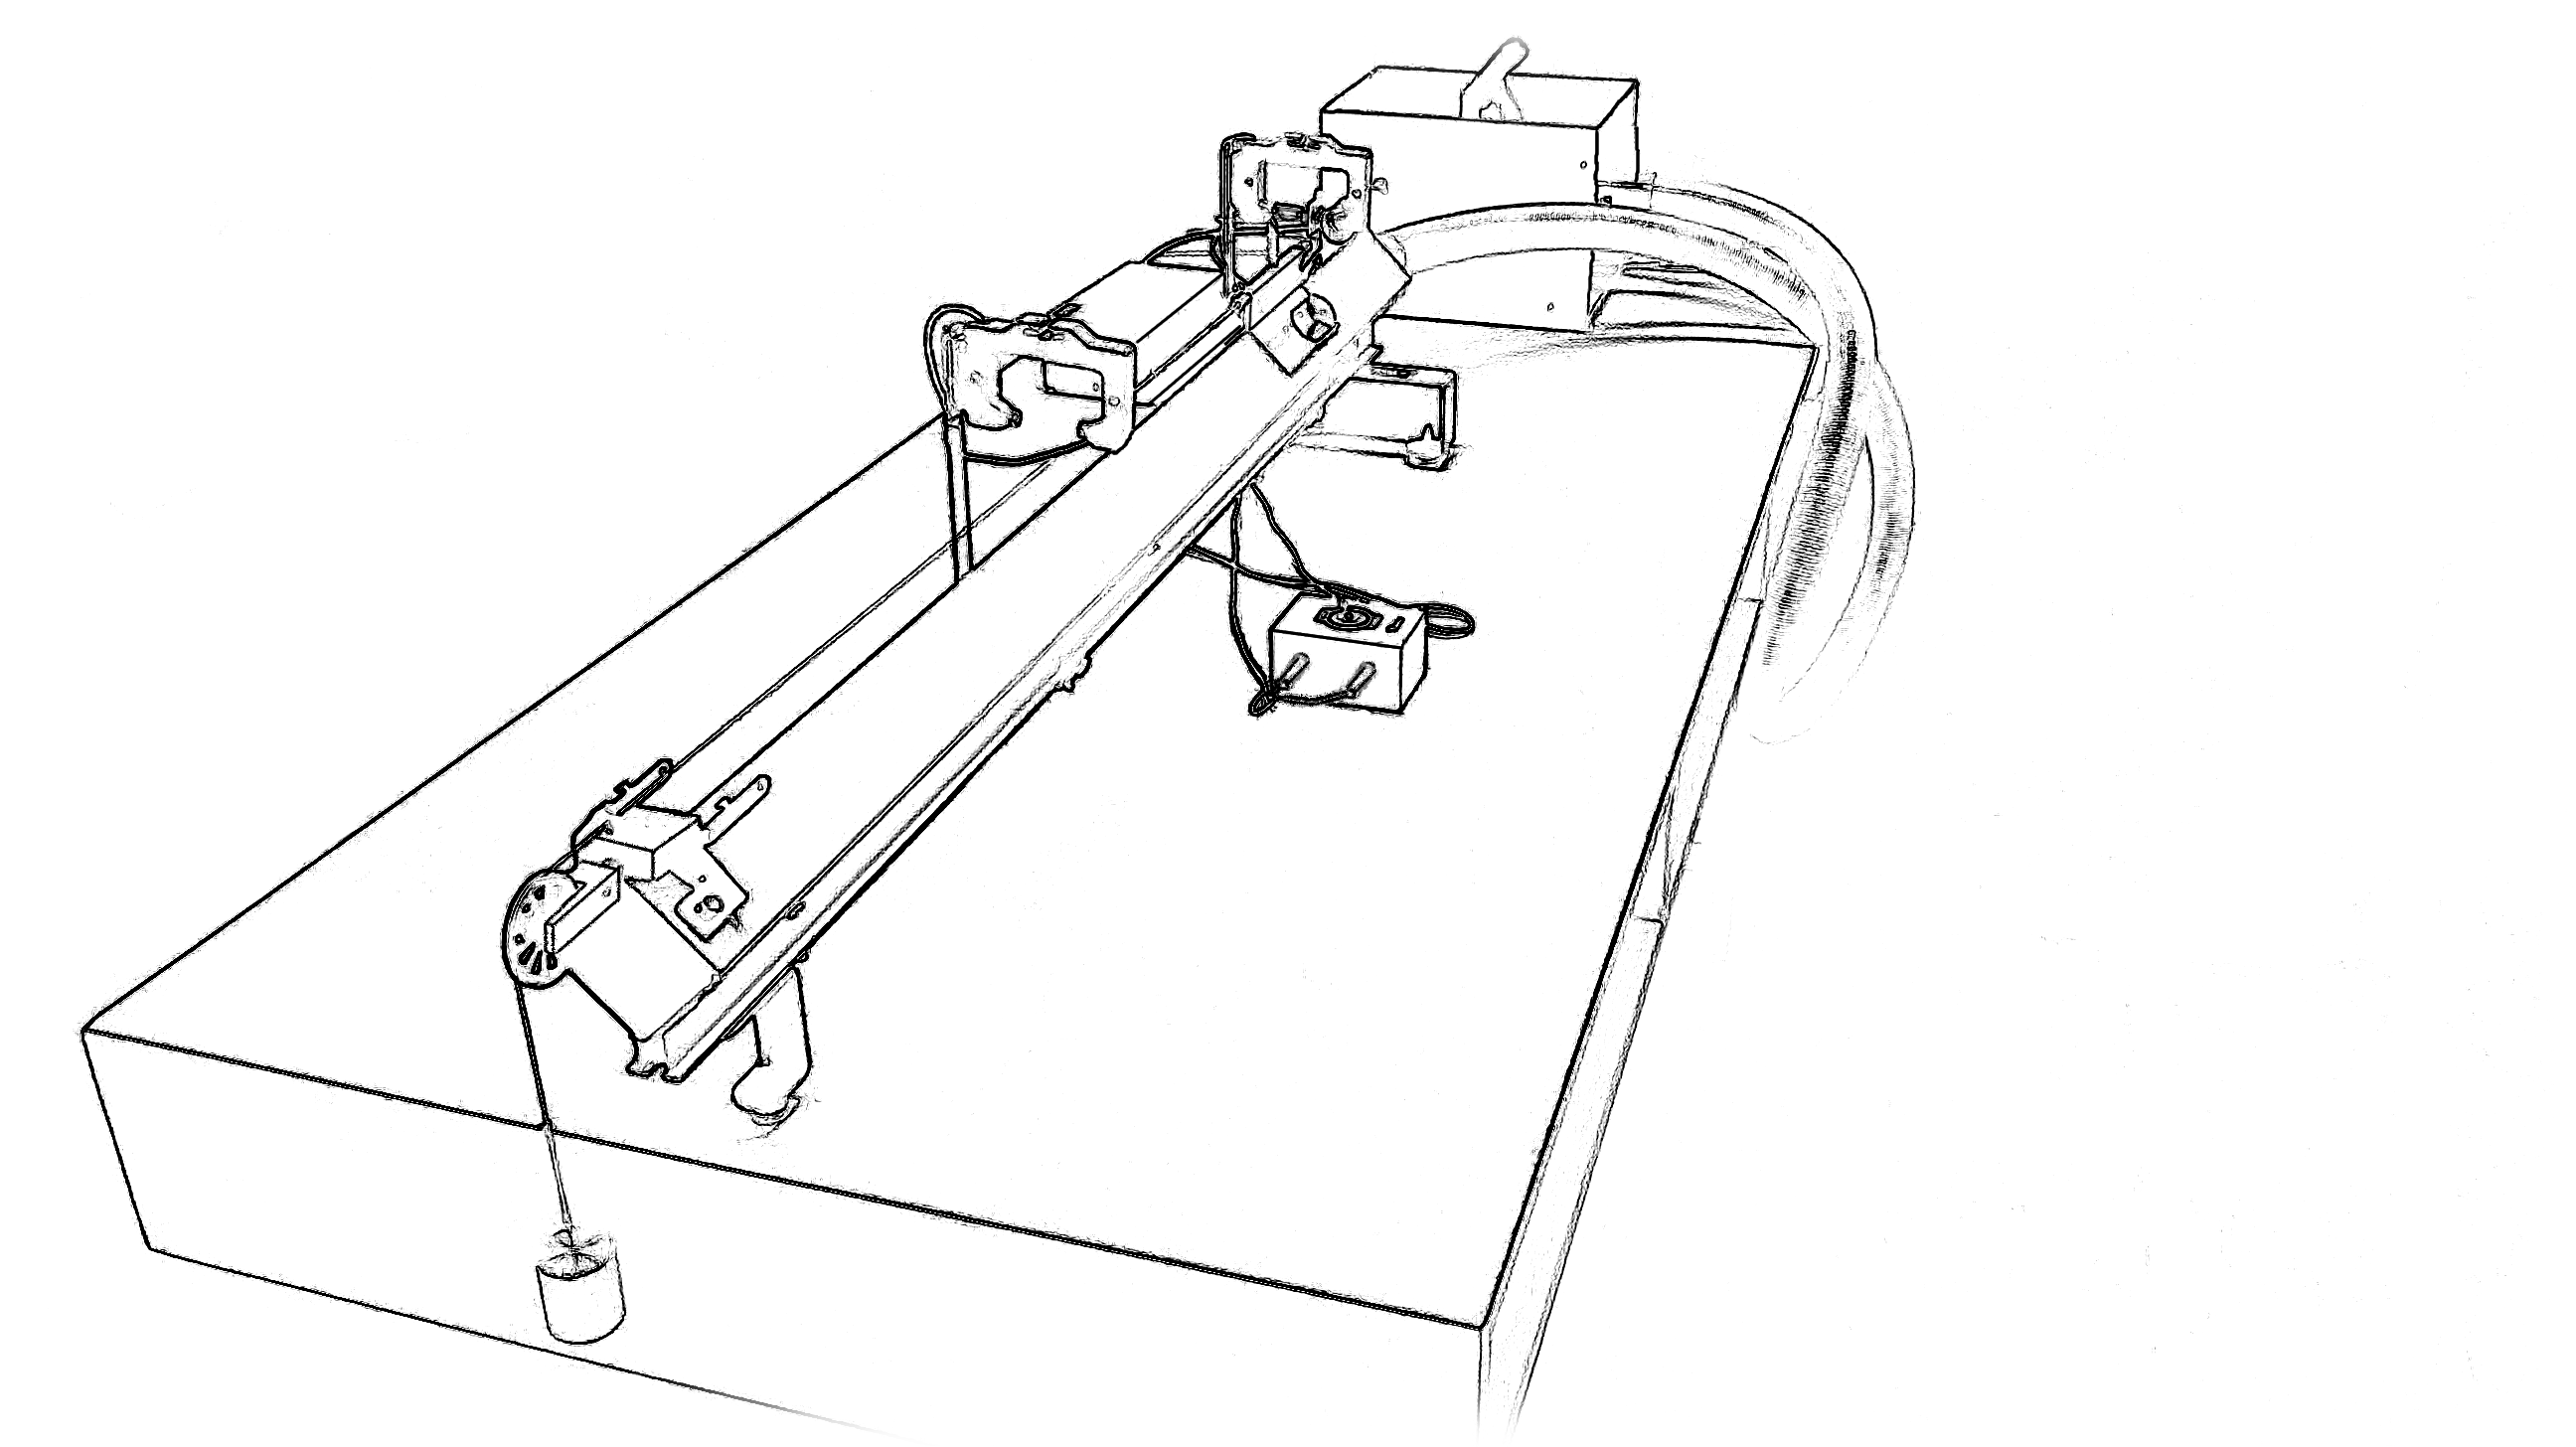
\includegraphics[width=\textwidth]{Ilustrations/TrilhoAr.png}
\caption{Objeto se movendo horizontalmente em um trilho de ar, submetido a uma aceleração devida ao objeto que cai.}
\label{FigTrilhoDeAr}
\end{figure}


%%%%%%%%%%%%%%%%%%%%%%%%%%%%%%%%%%%%%%%%%%%%%%%%%%
\subsection{Análise através das Leis de Newton}
%%%%%%%%%%%%%%%%%%%%%%%%%%%%%%%%%%%%%%%%%%%%%%%%%%

\begin{marginfigure}
\begin{tikzpicture}[>=Stealth,
     interface/.style={
        % superfície
        postaction={draw,decorate,decoration={border,angle=-45,
                    amplitude=0.2cm,segment length=2mm}}},
    ]

	% mesa
	\draw[interface] (0,0) -- (3,0);
	\draw[interface] (3,0) -- (3,-1);
	
	% roldana	
	\draw (3.3,0.05) circle[radius = 0.2];
	\draw[fill] (3.3,0.05) circle[radius = 0.05];
	\draw[fill] (2.6,0.1) rectangle (3.3,0);
	\draw[fill] (2.7,0.1) circle[radius = 0.05];
	\draw[fill] (2.9,0.1) circle[radius = 0.05];
	\draw[fill, white] (3.3,0.05) circle[radius = 0.02];
	
	% bloco superior
	\node[draw, densely dotted, circle, scale = 0.8] (b1) at (0.3,0.7) {1};
	\draw[pattern = north west lines, pattern color = gray, draw = gray] (0.5,0) rectangle +(1,0.5);
	\draw (1.5,0.25) -- (3.3,0.25);
	\draw[->, thick] (1,0) -- +(0,-1) node[left]{$\vec{P}_1$};
	\draw[->, thick] (1.5,0.25) -- +(0.5,0) node[above]{$\vec{T}$};
	\draw[->, thick] (1,0.5) -- +(0,1) node[left]{$\vec{N}$};
	
	% bloco inferior
	\node[draw, densely dotted, circle, scale = 0.8] (b2) at (3.1,-1.9) {2};
	\draw (3.5,0.05) -- +(0,-1);
	\draw[pattern = north west lines] (3.3,-0.95) rectangle +(0.4,-0.8);
	\draw[->, thick] (3.5,-0.95) -- +(0,0.5) node[right]{$\vec{T}$};
	\draw[->, thick] (3.5,-1.75) -- +(0,-0.75) node[right]{$\vec{P}_2$};
	
	% Coordenadas
	\draw[->, dashed] (0,0.25) -- (2.5,0.25) node[above]{$x_1$};
	\draw[->, dashed] (1,-1.5) -- (1,2) node[below right]{$y_1$};
	
	\draw[<-, dashed] (3.5, -1.35) +(0,2.25) node[below right]{$y_2$} -- +(0,-1.5);
	\draw[->, dashed] (3.5,-1.35)+(-1,0) -- +(1,0) node[below left]{$x_2$};
\end{tikzpicture}
\caption{Neste sistema, os blocos têm acelerações em eixos diferentes, porém ---~devido ao fato de que eles estão ligados por um fio inextensível~---, temos que $a_{1,x} = -a_{2,y}$.\label{Fig:MaquinaAtwoodHoriz}}
\end{marginfigure}

Analisando cada um dos objetos separadamente através da segunda lei de Newton:
\begin{description}
    \item[Bloco 1:] Aplicando a Segunda Lei de Newton para cada eixo:
        \begin{description}
            \item[Eixo $x_1$:]
                \begin{align}
                    F_{R, x_1} &= m_1 a_{1,x_1} \\
                    T & = m_1 a_{1,x_1}. \label{Eq:AtwoodHorizX1}
                \end{align}
            \item[Eixo $y_1$:]
                \begin{align}
                    F_{R, y_1} &= m_1 a_{1,y_1} \\
                    N_1 - P_1 &= m_1 a_{1,y_1} \\
                    N_1 - P_1 &= 0 \\
                    N_1 = P_1.
                \end{align}
        \end{description}
    \item[Bloco 2:] Novamente, aplicando a Segunda Lei de Newton para cada eixo:
        \begin{description}
            \item[Eixo $x_2$:] Não há nenhuma força/componente nesse eixo.
            \item[Eixo $y_2$:]
                \begin{align}
                    F_{R, y_2} &= m_2 a_{2,y_2} \\
                    T - P_2 &= m_2 a_{2,y_2}. \label{Eq:AtwoodHorizY2}
                \end{align}
        \end{description}
\end{description}

Para determinar a aceleração e a tensão, precisamos resolver o sistema de equações formado pelas expressões \eqref{Eq:AtwoodHorizX1} e \eqref{Eq:AtwoodHorizY2}. No entanto, temos três incógnitas: $a_{1,x}$, $a_{2,y}$ e $T$. Para que possamos resolver este sistema, precisamos de mais uma equação: a relação entre as acelerações. A aceleração do bloco 1 será no sentido positivo do eixo $x_1$, enquanto a aceleração do bloco 2 será no sentido negativo do eixo $y_2$. Se o fio é inextensível, podemos afirmar que o módulo dessas duas acelerações é o mesmo, o que nos leva à equação
\begin{equation}\label{Eq:AtwoodHorizRelAcel}
    a_{1,x} = - a_{2,y}.
\end{equation}
%
Assim
\begin{equation}
\begin{system}
T & = m_1 a_{1,x_1} \\
T - P_2 &= m_2 a_{2,y_2} \\
a_{1,x} &= - a_{2,y}. \\
\end{system}
\end{equation}
%
Se fizermos $a_{1,x_1} \equiv a$, pois estamos determinando o módulo da aceleração de cada bloco, podemos reescrever o sistema acima como
\begin{equation}
\begin{system}
T & = m_1 a \\
T - P_2 &= -m_2 a,
\end{system}
\end{equation}
%
o que resulta, a partir da soma da primeira equação com o negativo da segunda equação, em
\begin{align}
    T - T + P_2 &= m_1 a + m_2 a \\
    m_2 g &= (m_1 + m_2) a.
\end{align}
%
Finalmente, temos para a aceleração\footnote{Note que a fração é adimensional e que $g$ tem dimensão de aceleração. Consequentemente, o resultado tem as dimensões corretas.}
\begin{equation}\label{Eq:MaquinaAtwoodHorizResultAcel}
    a = \frac{m_2}{m_1+m_2} g.
\end{equation}

Para obtermos a tensão, basta retornar às equações do sistema e substituir o resultado para a aceleração. Fazendo isso com a primeira equação do sistema, temos
\begin{align}
    T &= m_1 a\\
    &= \frac{m_1m_2}{m_1+m_2} g. \label{Eq:MaquinaAtwoodHorizResultTensao}
\end{align}

Portanto, conhecendo o valor das massas dos dois objetos, temos condições de calcular a aceleração do sistema.

%%%%%%%%%%%%%%%%%%%%%%%%%%%%%%%%%%%%%%%%%%%%%%%%%%%%%%%%%%%
\subsection{Análise através das equações da cinemática.}
%%%%%%%%%%%%%%%%%%%%%%%%%%%%%%%%%%%%%%%%%%%%%%%%%%%%%%%%%%%

Uma outra forma de análise do sistema é através das equações da cinemática. Se formos capazes de medir a distância percorrida por qualquer um dos blocos e pudermos cronometrar o tempo necessário para realizar tal deslocamento, podemos extrair a aceleração dos dados utilizando a fórmula para o deslocamento de um objeto submetido a uma aceleração constante, isto é,
	\begin{equation}
		\Delta x = v_0 t + \frac{1}{2} at^2
	\end{equation}

Como podemos iniciar a cronometragem assim que o objeto começa a se mover, podemos eliminar a velocidade inicial $v_0$. Assim
\begin{equation}
	\Delta x = \frac{1}{2} at^2.
\end{equation}

Podemos calcular a aceleração a partir de um valor qualquer de deslocamento e do tempo correspondente. No entanto, o mais adequado é realizar uma série de medidas e utilizar o método dos mínimos quadrados para o conjunto de dados linearizado. Fazendo uma linearização, obtemos a seguinte relação entre a equação da reta e a equação acima:
\begin{align}
	y &= \Delta x \\
	A &= 0 \\
	B &= a/2 \\
	x &= t^2.
\end{align}
%
Podemos então calcular o coeficiente angular através de uma regressão linear dos dados obtidos para o deslocamento e para o tempo ao quadrado e obter um valor de aceleração independente daquele calculado através das leis de Newton. Isso possibilitará que comparemos os valores obtidos, testando assim a validade de tais leis.

%%%%%%%%%%%%%%%%%%%%%%%%%%%%%%%%%%%%%%%%%%%%%%%%%%%%%%%%%%%%%%%%%%%%%%%%%%%%%%%
\section{Experimento}
%%%%%%%%%%%%%%%%%%%%%%%%%%%%%%%%%%%%%%%%%%%%%%%%%%%%%%%%%%%%%%%%%%%%%%%%%%%%%%%

Vamos usar o aparato descrito na Seção~\ref{Sec:MaquinaDeAtwood} para determinar a aceleração através dos valores para a massa suspensa e para a massa do ``carrinho'' que deslisa sobre o trilho de ar. Além disso, vamos verificar o tempo necessário para que o carrinho percorra diversos valores de distância, sempre partindo do repouso, o que nos permitirá determinar a aceleração também através da cinemática. Poderemos então comparar os valores obtidos através dos dois métodos, verificando a validade das Leis de Newton.

%%%%%%%%%%%%%%%%%%%%%%
\subsection{Objetivos}
%%%%%%%%%%%%%%%%%%%%%%

\begin{itemize}
     \item Verificar a validade das Leis de Newton;
	 \item Linearizar o conjunto de dados obtidos e obter os valores de $A$ e $B$ da equação da reta correspondente;
	 \item Relacionar as variáveis cinemáticas às constantes da equação da reta;
     \item Calcular a aceleração do sistema através do valor do coeficiente angular ($B$) da reta;
     \item Elaborar um gráfico $\Delta x \times t$ dos pontos experimentais;
	 \item Elaborar um gráfico $\Delta x \times t^2$ dos pontos experimentais e adicionar a ele a reta obtida através da regressão linear.
\end{itemize}

%%%%%%%%%%%%%%%%%%%%%%%%%%%%%%%%%%%%%%%%%%%%%%%%%%%%%%%%%%%%%%%%%%%%%%%%%%%%%%%
\section{Material Necessário}
%%%%%%%%%%%%%%%%%%%%%%%%%%%%%%%%%%%%%%%%%%%%%%%%%%%%%%%%%%%%%%%%%%%%%%%%%%%%%%%

\begin{itemize}
	\item Conjunto de trilho de ar com sensores e cronômetro;
	\item Gancho e anilhas;
	\item Balança;
\end{itemize}

%%%%%%%%%%%%%%%%%%%%%%%%%%%%%%%%%%%%%%%%%%%%%%%%%%%%%%%%%%%%%%%%%%%%%%%%%%%%%%%
\section{Procedimento Experimental}
%%%%%%%%%%%%%%%%%%%%%%%%%%%%%%%%%%%%%%%%%%%%%%%%%%%%%%%%%%%%%%%%%%%%%%%%%%%%%%%

\begin{enumerate}
	\item Afira as massas do ``carrinho'' que se desloca sobre o trilho de ar e do conjunto formado pelo gancho e pelas anilhas. Anote os valores obtidos na Tabela~\ref{TabelaDadosLeisDeNewton}.
	\item Posicione o primeiro sensor imediatamente após a região do carrinho que ativa o sensor, de forma a garantir que a velocidade inicial seja nula;
	\item Posicione o segundo sensor a uma distância de cerca de \np[cm]{8,00} após o primeiro.
	\item Libere o carrinho e anote os valores obtidos de tempo e de distância percorrida na Tabela~\ref{TabelaDadosLeisDeNewton}.
	\item Desloque o segundo sensor distanciando-o mais \np[cm]{4,00} do primeiro.
	\item Libere o carrinho novamente e anote os novos valores de tempo e de distância percorrida na Tabela~\ref{TabelaDadosLeisDeNewton}.
	\item Repita os dois itens acima com tantos dados quanto possível. Observe que conforme o conjunto de anilhas desce, ele eventualmente colide com o chão. \textbf{A colisão com o chão só pode acontecer após o carrinho ter passado pelo segundo sensor.} Portanto, o valor máximo de distância entre os sensores estará limitado por esse fator. 
\end{enumerate}

%%%%%%%%%%%%%%%%%%%%%%%%%%%%%%%%%%%%%%%%%%%%%%%%%%%%%%%%%%%%%%%%%%%%%%%%%%%%%%%
%%%%%%%%%%%%%%%%%%%%%%%%%%%%%%%%%%%%%%%%%%%%%%%%%%%%%%%%%%%%%%%%%%%%%%%%%%%%%%%
%%%%%%%%%%%%%%%%%%%%%%%%%%%%%%%%%%%%%%%%%%%%%%%%%%%%%%%%%%%%%%%%%%%%%%%%%%%%%%%
%%%%%%%%%%%%%%%%%%%%%%%%%%%%%%%%%%%%%%%%%%%%%%%%%%%%%%%%%%%%%%%%%%%%%%%%%%%%%%%
\cleardoublepage

\noindent{}{\huge\textit{Leis de Newton}}

\vspace{15mm}

\begin{fullwidth}
\noindent{}\makebox[0.6\linewidth]{Turma:\enspace\hrulefill}\makebox[0.4\textwidth]{  Data:\enspace\hrulefill}
\vspace{5mm}

\noindent{}\makebox[0.6\linewidth]{Aluno(a):\enspace\hrulefill}\makebox[0.4\textwidth]{  Matrícula:\enspace\hrulefill}

\noindent{}\makebox[0.6\linewidth]{Aluno(a):\enspace\hrulefill}\makebox[0.4\textwidth]{  Matrícula:\enspace\hrulefill}

\noindent{}\makebox[0.6\linewidth]{Aluno(a):\enspace\hrulefill}\makebox[0.4\textwidth]{  Matrícula:\enspace\hrulefill}

\noindent{}\makebox[0.6\linewidth]{Aluno(a):\enspace\hrulefill}\makebox[0.4\textwidth]{  Matrícula:\enspace\hrulefill}

\noindent{}\makebox[0.6\linewidth]{Aluno(a):\enspace\hrulefill}\makebox[0.4\textwidth]{  Matrícula:\enspace\hrulefill}
\end{fullwidth}

\vspace{5mm}

%%%%%%%%%%%%%%%%%%%%%%%%%%%%%%%%%%%%%%%%%%%%%%%%%%%%%%%%%%%%%%%%%%%%%%%%%%%%%%%
\section{Questionário}
%%%%%%%%%%%%%%%%%%%%%%%%%%%%%%%%%%%%%%%%%%%%%%%%%%%%%%%%%%%%%%%%%%%%%%%%%%%%%%%

\begin{question}[type={exam}]{1}
Apresente os resultados de maneira clara e organizada. Mostre os cálculos requisitados de maneira clara e sucinta, evidenciando o raciocínio desenvolvido.
\end{question}

\begin{question}[type={exam}]{1}
Preencha as colunas de dados experimentais das tabelas com o número adequado de algarismos significativos e unidades.
\end{question}

\begin{question}[type={exam}]{2.5}
Elabore\footnote{Na verdade, em ambos os casos o deslocamento $\Delta x$ é a variável independente. Por questões didáticas, no entanto, estamos optando por tratar o tempo como variável independente.} um gráfico $\Delta x \times t$ dos pontos experimentais e um gráfico $\Delta x \times \tau$, onde $\tau = t^2$.
\end{question}

\begin{question}[type={exam}]{2}
Através dos gráficos elaborados no item anterior, podemos verificar qual dos dois conjuntos de dados segue uma tendência linear. Para o conjunto de dados linear, obtenha os valores de $A$, $B$ e $r^2$ da melhor reta correspondente, isto é, faça a regressão linear dos dados experimentais. Adicione essa reta ao gráfico correspondente e coloque a equação da reta, juntamente com o coeficiente $r^2$ na legenda.
\end{question}

\begin{question}[type={exam}]{1.5}
Relacione as variáveis cinemáticas às constantes da equação da reta. Calcule através do coeficiente angular $B$ qual é a aceleração do sistema.
\end{question}

\begin{question}[type={exam}]{1}
Compare o valor o valor obtido para a aceleração com o valor dado pelas leis de Newton através do \emph{erro percentual} dado pela expressão\footnote[][-5mm]{A expressão para o erro percentual é geral e costuma ser escrita como %
\begin{minipage}{\linewidth} %
\begin{align*} %
    E_\% = \left|\frac{x - x_{\textrm{Ref}}}{x_{\textrm{Ref}}}\right| \times 100, %
\end{align*} %
\vspace{0.1mm}
\end{minipage} %
%
onde $x$ é uma medida qualquer que queremos comparar com um valor de referência $x_{\text{Ref}}$.}
\begin{equation}
	E_\% = \left|\frac{a - a_{\textrm{Ref}}}{a_{\textrm{Ref}}}\right| \times 100,
\end{equation}
%
onde $a_{\textrm{Ref}}$ é o valor obtido para a aceleração através das Leis de Newton e $a$ é o valor obtido através do coeficiente $B$ da regressão linear.
\end{question}

\begin{question}[type={exam}]{1}
Inverta a Equação~\eqref{Eq:MaquinaAtwoodHorizResultAcel} e isole a gravidade. Use o valor da aceleração obtido através dos dados cinemáticos e calcule o valor de $g$. Utilize a fórmula para o erro percentual e calcule $E_\%$ com relação ao valor $g=\np[m/s^2]{9,8}$.
\end{question}

\vfill
%%%%%%%%%%%%%%%%%%%%%%%%%%%%%%%%%%%%%%%%%%%%%%%%%%%%%%%%%%%%%%%%%%%%%%%%%%%%%%%
\pagebreak
\section{Tabelas}
%%%%%%%%%%%%%%%%%%%%%%%%%%%%%%%%%%%%%%%%%%%%%%%%%%%%%%%%%%%%%%%%%%%%%%%%%%%%%%%

\begin{table}[!ht]
\centering
\begin{tabular}{lp{25mm}p{25mm}p{25mm}l}
\toprule
	& \multicolumn{3}{l}{\textbf{Massas}} \\
	\cmidrule{2-4}
	& \multicolumn{2}{l}{Carrinho \cellcolor[gray]{0.89}} & \cellcolor[gray]{0.92} \\
	& \multicolumn{2}{l}{Gancho e anilhas \cellcolor[gray]{0.95}} & \cellcolor[gray]{0.97}\\
	\cmidrule{2-4}
\\
	&\multicolumn{3}{l}{\textbf{Dados experimentais}} \\
	\cmidrule{2-4}
	& $x_i$ & $x_f$ & $t$ & \\
	\cmidrule{2-4}
	& \cellcolor[gray]{0.89} & \cellcolor[gray]{0.92} & \cellcolor[gray]{0.89} \\
	& \cellcolor[gray]{0.95} & \cellcolor[gray]{0.97} & \cellcolor[gray]{0.95} \\
	& \cellcolor[gray]{0.89} & \cellcolor[gray]{0.92} & \cellcolor[gray]{0.89} \\
	& \cellcolor[gray]{0.95} & \cellcolor[gray]{0.97} & \cellcolor[gray]{0.95} \\
	& \cellcolor[gray]{0.89} & \cellcolor[gray]{0.92} & \cellcolor[gray]{0.89} \\
	& \cellcolor[gray]{0.95} & \cellcolor[gray]{0.97} & \cellcolor[gray]{0.95} \\
	& \cellcolor[gray]{0.89} & \cellcolor[gray]{0.92} & \cellcolor[gray]{0.89} \\
	& \cellcolor[gray]{0.95} & \cellcolor[gray]{0.97} & \cellcolor[gray]{0.95} \\
	& \cellcolor[gray]{0.89} & \cellcolor[gray]{0.92} & \cellcolor[gray]{0.89} \\
	& \cellcolor[gray]{0.95} & \cellcolor[gray]{0.97} & \cellcolor[gray]{0.95} \\
	& \cellcolor[gray]{0.89} & \cellcolor[gray]{0.92} & \cellcolor[gray]{0.89} \\
	& \cellcolor[gray]{0.95} & \cellcolor[gray]{0.97} & \cellcolor[gray]{0.95} \\
	& \cellcolor[gray]{0.89} & \cellcolor[gray]{0.92} & \cellcolor[gray]{0.89} \\
	& \cellcolor[gray]{0.95} & \cellcolor[gray]{0.97} & \cellcolor[gray]{0.95} \\
	& \cellcolor[gray]{0.89} & \cellcolor[gray]{0.92} & \cellcolor[gray]{0.89} \\
	& \cellcolor[gray]{0.95} & \cellcolor[gray]{0.97} & \cellcolor[gray]{0.95} \\
	\cmidrule{2-4}
\\
	& \multicolumn{3}{l}{\textbf{Valores calculados}} \\
	\cmidrule{2-3}
	& $\Delta x$ & $t^2$ \\
	\cmidrule{2-3}
	& \cellcolor[gray]{0.89} & \cellcolor[gray]{0.92} \\
	& \cellcolor[gray]{0.95} & \cellcolor[gray]{0.97} \\
	& \cellcolor[gray]{0.89} & \cellcolor[gray]{0.92} \\
	& \cellcolor[gray]{0.95} & \cellcolor[gray]{0.97} \\
	& \cellcolor[gray]{0.89} & \cellcolor[gray]{0.92} \\
	& \cellcolor[gray]{0.95} & \cellcolor[gray]{0.97} \\
	& \cellcolor[gray]{0.89} & \cellcolor[gray]{0.92} \\
	& \cellcolor[gray]{0.95} & \cellcolor[gray]{0.97} \\
	& \cellcolor[gray]{0.89} & \cellcolor[gray]{0.92} \\
	& \cellcolor[gray]{0.95} & \cellcolor[gray]{0.97} \\
	& \cellcolor[gray]{0.89} & \cellcolor[gray]{0.92} \\
	& \cellcolor[gray]{0.95} & \cellcolor[gray]{0.97} \\
	& \cellcolor[gray]{0.89} & \cellcolor[gray]{0.92} \\
	& \cellcolor[gray]{0.95} & \cellcolor[gray]{0.97} \\
	& \cellcolor[gray]{0.89} & \cellcolor[gray]{0.92} \\
	& \cellcolor[gray]{0.95} & \cellcolor[gray]{0.97} \\
	\cmidrule{2-3}
\bottomrule
\end{tabular}
\caption{Valores de tempo e deslocamento para o MRUV.}
\label{TabelaDadosLeisDeNewton}
\end{table}
